Lattice methods are computational techniques used to value options and other derivatives by constructing a lattice, essentially a grid-like representation of the underlying asset's possible price movements over discrete time intervals \citep{coxOptionPricingSimplified1979a}. In a lattice, each node represents a possible price level of the underlying asset at a specific point in time. Starting from the initial price, the lattice evolves by considering possible upward and downward movements based on the asset's volatility.

Pricing barrier options can be challenging due to the added complexity introduced by the barrier conditions. In a lattice, the barrier levels can be incorporated into the calculations by adjusting the probabilities of price movements, which will be analysed with the Bino-Trinomial model.

At each step of the tree, the asset price can over the time step $\Delta t$ either move up by a fixed amount $u$ with a probability $p_u$ or decrease by a fixed amount $d$ with a probability $p_d = 1 - p_u$. We assume there are $n$ steps in the tree.

We define $i$ and $j$ as the number of price and time steps until the considered node $(j, i)$. As a consequence, the number of paths that lead to the node is $\binom{j}{i}$ with probability $\binom{j}{i} p_u^i p_d^{j-i}$. At each time point $j$, the random variable $S_n$ (describing the stock price) takes value on $\{S_0 u^j, S_0 u^{j-1} d, \ldots, S_0 d^j\}$. The discrete stock price process follows
\[
	S_n = S_0 \prod_{i=1}^n \xi_i
\]
where $\xi_i$ are iid random variables defined as follows:
\[
	\xi_i =
	\begin{cases}
		u & \text{with probability } q_u \\
		d & \text{with probability } q_d
	\end{cases}
\]

A simple approach uses backward induction to price the option with a binomial tree.

\begin{figure}[H]
	\centering
	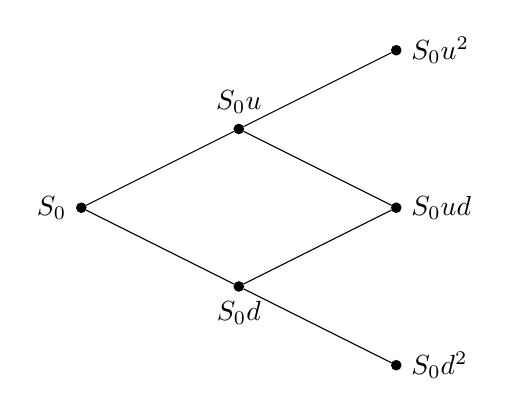
\begin{tikzpicture}[scale=2]
		% Nodes with dots
		\node[draw, fill=black, circle, inner sep=1.2pt, label=left:{$S_0$}] (S0) at (0,0) {};
		\node[draw, fill=black, circle, inner sep=1.2pt, label=above:{$S_0u$}] (Su) at (1,0.5) {};
		\node[draw, fill=black, circle, inner sep=1.2pt, label=below:{$S_0d$}] (Sd) at (1,-0.5) {};
		\node[draw, fill=black, circle, inner sep=1.2pt, label=right:{$S_0u^2$}] (Suu) at (2,1) {};
		\node[draw, fill=black, circle, inner sep=1.2pt, label=right:{$S_0ud$}] (Sud) at (2,0) {};
		\node[draw, fill=black, circle, inner sep=1.2pt, label=right:{$S_0d^2$}] (Sdd) at (2,-1) {};

		% Edges
		\draw[-] (S0) -- (Su);
		\draw[-] (S0) -- (Sd);
		\draw[-] (Su) -- (Suu);
		\draw[-] (Su) -- (Sud);
		\draw[-] (Sd) -- (Sud);
		\draw[-] (Sd) -- (Sdd);
	\end{tikzpicture}
	\caption{A two-step Binomial Tree}
	\label{fig:TwoStepBinomialTree}
\end{figure}

\begin{thm}{Backward Induction}{}
	Consider $V^j = e^{-r_d (n-j) \Delta t} \mathbb{E}[g(S_n) | \mathcal{F}_j]$, the time-$j$ fair value of the European call option. \emph{We have the following recursive algorithm:}
	\[
		V^j =
		\begin{cases}
			g(S_n)                                                & j = n      \\
			e^{-r_d \Delta t} \mathbb{E}[V^{j+1} | \mathcal{F}_j] & j \leq n-1
		\end{cases}
	\]
\end{thm}

The up and down factors $u$ and $d$, along with their corresponding probabilities, must match the first two moments of the price distribution. There are only two equations and three parameters to determine (knowing one probability $p_u$ also makes it possible to know $p_d = 1-p_u$). Cox-Ross-Rubinstein (CRR) set the additional equation to $ud = 1$. The CRR model has parameters:

\begin{align}
	u   & = e^{\sigma \sqrt{\Delta t}}          \\
	d   & = e^{-\sigma \sqrt{\Delta t}}         \\
	p_u & = \frac{e^{(r-q)\Delta t} - d}{u - d}
\end{align}

Under this configuration and with the previous theorem, we define the following recursive formula:
\begin{equation}
	V^j_i = e^{-r_d \Delta t} \left[ p_u V^{j+1}_{i+1} + p_d V^{j+1}_i \right]
\end{equation}

At the end of the recursive algorithm, we obtain the time-zero option value.\\
In the standard CRR tree, the local volatility is constant for each time step and converges to the input volatility as $n$ becomes large:
\begin{equation}
	\sigma^{j}_i = \frac{1}{\sqrt{\Delta t}} \sqrt{p_u p_d} \ln u^2
\end{equation}

\begin{thm}{Closed-Form Binomial Price for Vanilla Option}{}
	The price of a Vanilla option for an $n \in \mathbb{N}$ step tree is given by,
	\[
		V = e^{-r_d n \Delta t} \left[ \sum_{j=0}^{n} \binom{n}{j} p_u^j p_d^{n-j} V^j \right].
	\]
\end{thm}
\begin{xattention}
	One remark to make with that CRR model is that in some cases where $\sigma < |(r-q)/\sqrt{\Delta t}|$, negative probabilities can occur. First, it is inconsistent from a probability theory perspective, but additionally, it may prevent the model from capturing relevant events.
\end{xattention}

\begin{prop}{Cox-Ross-Rubinstein Valuation}{CRRValuation}
	For every $m = 1, 2, \dots, T$, the arbitrage price of a European call option at time $t = T - m$ is given by the Cox-Ross-Rubinstein valuation formula
	\begin{equation} \label{eq:CRRValuationFormula}
		C_{T-m} = S_{T-m} \sum_{j=a}^m \bincof{m}{j} \bar{p}^j (1 - \bar{p})^{m-j} - \frac{K}{\hat{r}^m} \sum_{j=a}^m \bincof{m}{j} p_*^j (1 - p_*)^{m-j},
	\end{equation}
	where $a = a_m(S_{T-m})$, $p_* = (\hat{r} - d)/(u-d)$ and $\bar{p} = p_* u / \hat{r}$. At time $t = T - m - 1$, the unique replicating strategy $\phi_{T-m-1} = (\alpha_{T-m-1}, \beta_{T-m-1})$ equals
	\begin{align*}
		\alpha_{T-m-1} & = \sum_{j=a^d}^m \bincof{m}{j} \bar{p}^j (1 - \bar{p})^{m-j} + \frac{\delta \Delta_m(u S_{T-m-1}, a^u)}{S_{T-m-1}(u-d)},                   \\
		\beta_{T-m-1}  & = - \frac{K}{\hat{r}^{m+1}} \sum_{j=a^d}^m \bincof{m}{j} p_*^j (1 - p_*)^{m-j} - \frac{\delta d \Delta_m(u S_{T-m-1}, a^u)}{\hat{r}(u-d)},
	\end{align*}
	where $a^d = a_m(d S_{T-m-1})$, $a^u = a_m(u S_{T-m-1})$ and $\delta = a^d - a^u$.
\end{prop}
